\chapter{Literature review}

\section{Natural Language Processing with Deep Learning}
It is non-negligible thing to unified fundamental knowledge in a Deep Learning architecture from Collobert et al. (2011) \cite{DBLP:journals/corr/abs-1103-0398}.
The work is cover various task on Natural Language Processing (NLP) problem including part-of-speech tagging, chunking, named entity recognition (NER), and semantic role labeling.
There are only two models introduced in this work which are sentence approach network and window approach network.
The window approach network consider fixed size window of words around one word.
Given that the tag of a word depends mainly on its neighboring, the window approach network usually provides a good result on most tasks such as part-of-speech tagging, chunking, name entity detection.
However, for semantic role labeling task, a tag of each word usually depends on a verb.
Given that a verb of one word could be placed outside the window, the tag of that word would be incorrect.
The word approach network consists with a predicted target word and its neighbor.
For example, if the window size equal to two, to predict \textbf{W\textsubscript{n}}, we would required \textbf{W\textsubscript{n-2}}, \textbf{W\textsubscript{n-1}}, \textbf{W\textsubscript{n}}, \textbf{W\textsubscript{n+1}}, and \textbf{W\textsubscript{n+2}} as input for this network as 1D tensor of word indexes.
This input is then mapped to an embedding layer which equivalence to a lookup table to replace these word indexes to 2D tensor features.
The output from embedding layer then become an input for the next linear layer.
Finally, the linear layer output is used as the input of a classifier layer to determined the tag of a word located in the center of the window.
Figure \ref{fig:window_approach_network} portrayed a simplest sample of a model to predict a tag of a second word (\textbf{W\textsubscript{2}}) in sentence \textbf{i} (\textbf{S\textsubscript{i}}) with window size equal to one.
As for sentence approach, the whole \textbf{S\textsubscript{i}} is used to predict each word tags using a convolution layer instead of a linear layer as illustrates in Figure \ref{fig:sentence_approach_network}. The convolution layer extracts features of each word in the sentence as 2D tensor. 
This convolution layer is introduced by Waibel et al (1989) \cite{Waibel1989PhonemeRU} called Time Delay Neural Networks (TDNNs).
Finally, each word features then used as input for the classifier layer individually to determine a tag of each input word in that sentence. 
This model is well-known and is proofed to be effective in various NLP tasks. 
Hence, it has usually been used to forge a baseline for multiple tasks in NLP research field.
\begin{figure}[!h]
  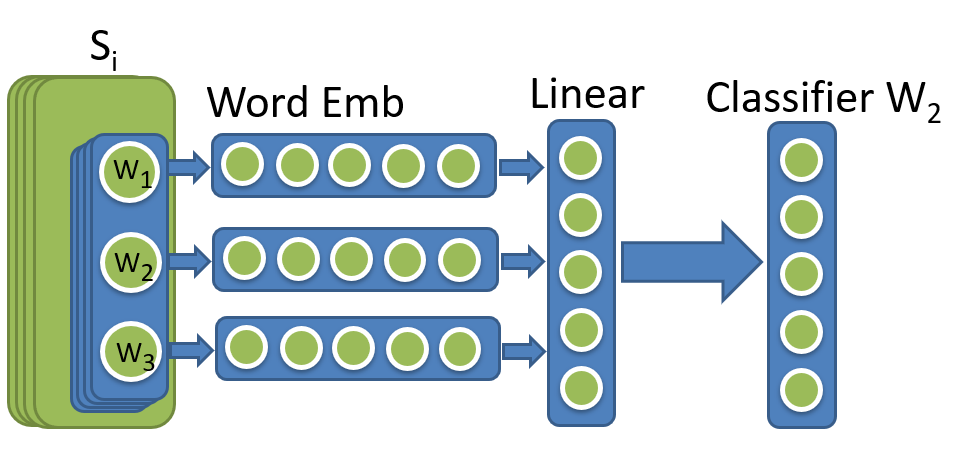
\includegraphics[scale=0.5]{window_approach_network.png}
  \caption{Window approach network.}
  \label{fig:window_approach_network}
\end{figure}
\begin{figure}[!h]
  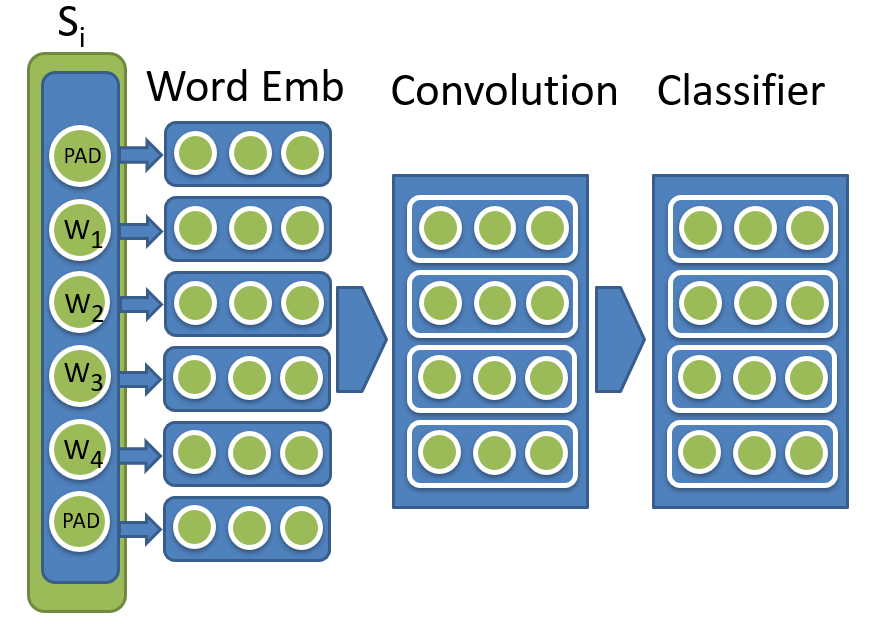
\includegraphics[scale=0.5]{sentence_approach_network.png}
  \caption{Sentence approach network.}
  \label{fig:sentence_approach_network}
\end{figure}


\section{Neural architectures for named entity recognition}
To illustrate a clear picture of each work, one should views the published model into three level separately: Character-Encoder level, Word-Encoder level, and Tag-Decoder level.
The process during Character-Encoder level are counted from the character feature look-up table to each word features are extracted from a sequence of characters.
The Word-Encoder level is a process from a creation of each word feature to an acquisition of each word hidden feature.
Finally, the Tag-Decoder level is the usage of each word hidden feature to clarify tag of each word using Conditional Random Field (CRF) proposed by Lafferty et al. (2001) \cite{Lafferty:2001:CRF:645530.655813}.
Since recently pioneered by Collobert et al. (2011) \cite{DBLP:journals/corr/abs-1103-0398} there are several works regarding NER task especially that based on his work. Huang et al. (2015) \cite{DBLP:journals/corr/HuangXY15} proposed a changed from Convolutional Neural Networks (CNN) proposed by Lecun et al. (1995) \cite{lecun1995convolutional} to a Long-Short Term Memory (LSTM) proposed by Hochreiter et al. (1997) \cite{DBLP:journals/neco/HochreiterS97} in the Word-Encoder level.
Introduce by Lample et al. (2016) \cite{DBLP:journals/corr/LampleBSKD16}, their word involve with a variant combination methods such as pretrain word using Skip-n-gram Word2Vec (Ling et al., 2015) \cite{DBLP:journals/corr/LingLMAADBT15}, dropout (Srivastava et al., 2014) \cite{JMLR:v15:srivastava14a}, LSTM , and CRF.
Their approach is separated into two aspects: LSTM-CRF and Stacked LSTMs.
However, the important distinction of their work is a feature extraction from character-level using Bidirectional LSTM (BiLSTM) proposed by Graves et al. (2005) \cite{graves2005framewise} instead of hand-engineering feature creation such as prefix and suffix.
The usage of character-level idea have been found useful for morphologically rich languages to handle an out of vocabulary problem that always occur.
The character-level output are concatenate with word presentation feature to form a full feature words which use as an input for LSTM layer of Word-Encoder level to achieve each word hidden feature.
Thus, the model can made a tag prediction of one word by using previous tags and the word own hidden feature.
The work has shown that the combination of LSTM-LSTM-CRF added with pre-train word embedding and dropout given the best result.
Similar work is done by Chiu et al. (2016) \cite{DBLP:journals/corr/ChiuN15} which replaced LSTM in the Character-Encoder level to CNN.
Yang et al. (2016) \cite{DBLP:journals/corr/YangSC16} also replaced the Character-Encoder and Word-Encoder levels with a Gate Recurrent Unit (GRU) proposed by Cho et al. (2014) \cite{DBLP:journals/corr/ChoMGBSB14} result in a GRU-GRU-CRF model.
In another aspects, the Tag-Decoder level is a main focus for Nguyen et al. (2016) \cite{DBLP:journals/corr/NguyenSDF16} where the use of a recurrent neural network (RNN) found by Hopfield (1982) \cite{hopfield1982neural} is introduced.
With this changed, when the number of entity types is enormous, the model could be train faster than CRF.
Later on, it has been demonstrated by Shen et al. (2017) \cite{DBLP:journals/corr/ShenYLKA17} that a usage of LSTM in Tag-Decoder level could outperform CRF.
His work introduced a changed in the Tag-Decoder that usually used CRF for NER task to LSTM while combining each word with Character-Encoder level approach.
Furthermore, with Active learning algorithm, a model proof to be able to manipulate its learning process by choosing contexts in training set to learn by itself, which minimize amount of sampling for training.
Compare with other models, his LSTM-LSTM-LSTM achieve the highest F1-score.


\section{Weighted Cross-Entropy for imbalance data}

The total amount of name entity in our training data contains 190 classes excluding ``B-'', ``I-'', and ``O'' tags.
This leads to an imbalance label problem. Furthermore, NER task is usually fill with high ratio of O-Tags.
As a result, the training model will subsequently made an adjustment on O-Tags first to minimize the loss.
When this problem arise, the training model is bound to stuck in its local minima.
Thus, result in a model which could only predicted O-Tags correctly.
Therefore, we view that the weighted calculation for each tag in our categorical Cross-Entropy is a non-trivial matter and it could be solve similarly to a rare word detection problem.
There are some published which discussed about this in a keyword detection model proposed by Panchapagesan et al. (2016) \cite{DBLP:conf/interspeech/PanchapagesanSK16}, and Sun et al. (2017) \cite{DBLP:journals/corr/SunRTPFMMSV17}.

\section{Our work}
From the previous studying, even through, while the model which done in a more complicate method usually provide a better result, its also raise a question that could a compact one be able to achieve such a result.
Hence, an optimization of the model is the main focus of this work.
In term of optimization, our main contribution lays in various aspect such as a training duration, most needed feature, and an amount of epoch for training until model converge.
The author absolutely agree that the usage of Character-Encoder level cannot be neglect in the case such as Chinese characters (Kanji) could hold an important feature such as the location or person name.
There are various combination of Kanji and the training corpus obviously could not suffice all of its combination.
However, instead of the usage of LSTM at Character-Encoder level to a whole sentence like the other work.
The LSTM is applied at Character-Encoder level on a batch of set of word.
As Japanese language has no explicit word boundary markers in every sentence, the word segmentation is quite crucial and the Character-Encoder level should not deal with the whole string directly as the relationship between character should laid in their respective word only.
The main reason for not using BiLSTM on this layer is that, if the order of characters is changed, it would become a different word accordingly.
Therefore, the discernment on character ordering is automatically distinguished in the Word-Encoder level.
In additional, considering that usually Noun is a name entity, characters of a word which is not ``Noun'' could be neglected to improve training speed.
The Word-Encoder level is where the model applied a handcrafted feature: part-of-speech, and partial handcrafted feature: Japanese particle augmented to the output of Character-Encoder.
Finally, the Tag-Decoder layer, each tag is a final output which is a classifying result from an output of Word-Encoder and a previous tag as its LSTM input.
The model is portrayed and explained in detailed in the next section.
